\documentclass[tikz, border=3pt]{standalone}

\usepackage{tikz}
\usepackage{pgfplots}

\begin{document}
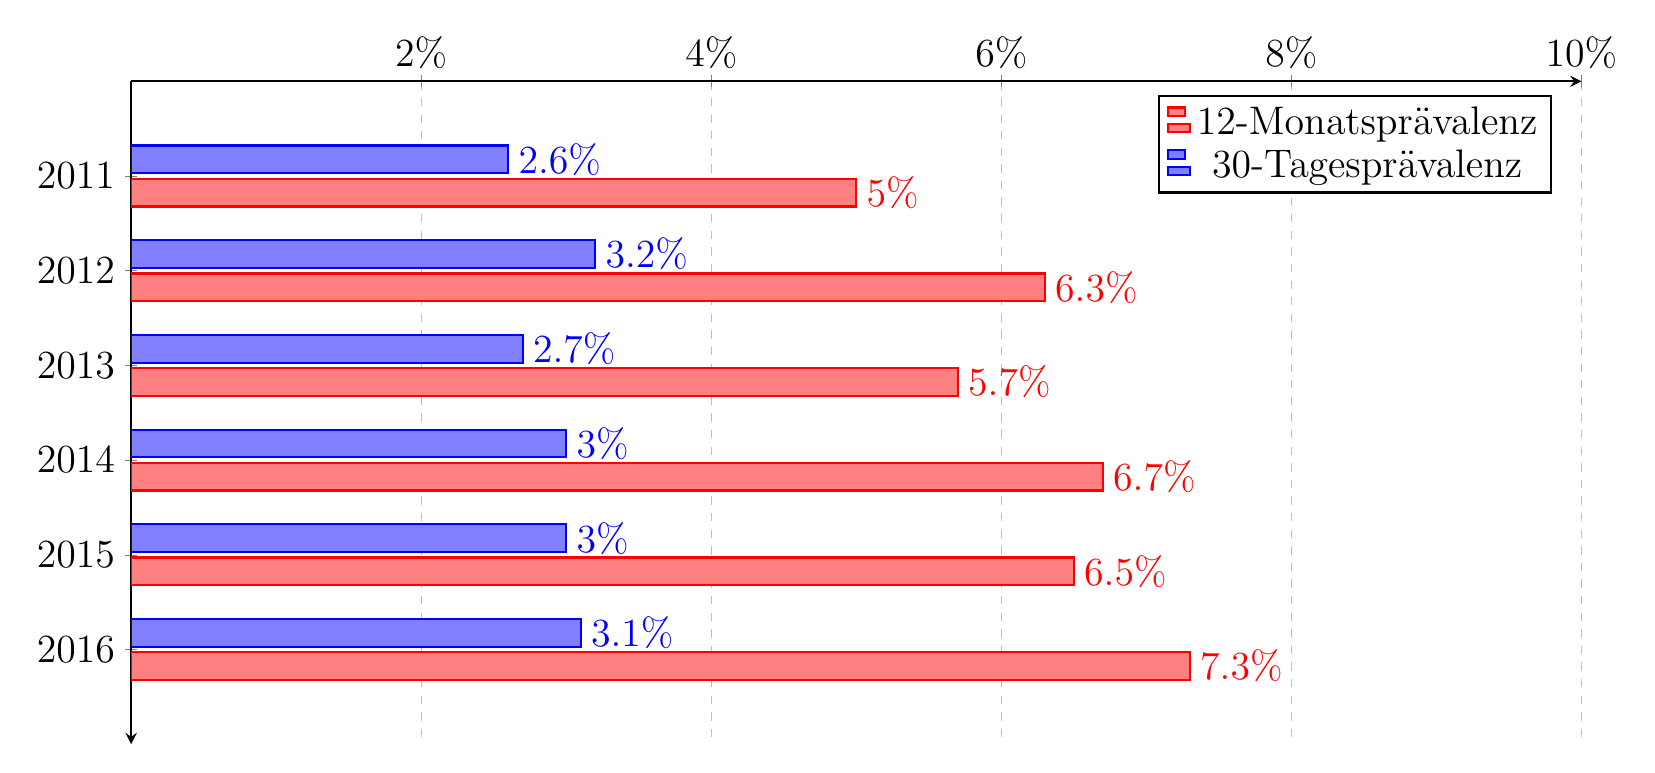
\begin{tikzpicture}

\begin{axis}[
	thick,
	xbar,
	xmin=0, xmax=10,
	ymin=0, ymax=7,
	width=20cm,
	height=10cm,
	xtick={2,4,6,8,10},
    ytick = {1,2,3,4,5,6},
	yticklabels={
		\Large 2011,
		\Large 2012,
		\Large 2013,
		\Large 2014,
		\Large 2015,
		\Large 2016
	},
	y dir=reverse,
	x tick label style={yshift=1mm,anchor=south},
	xticklabel={\Large\pgfmathprintnumber\tick\%},
	axis lines=middle,
    xmajorgrids,
    grid style={dashed}
]


	
% Cannabis
\addplot[ 
	color=red,
	fill=red!50!,
	bar width=10pt,
	nodes near coords=\Large\pgfmathprintnumber{\pgfplotspointmeta}\%,
] coordinates {
	(5.0, 1)
	(6.3, 2)
	(5.7, 3)
	(6.7, 4)
	(6.5, 5)
	(7.3, 6)
};

\addplot[ 
	color=blue,
	fill=blue!50!,
	bar width=10pt,
	nodes near coords=\Large\pgfmathprintnumber{\pgfplotspointmeta}\%,
] coordinates {
	(2.6, 1)
	(3.2, 2)
	(2.7, 3)
	(3.0, 4)
	(3.0, 5)
	(3.1, 6)
};

\legend{\Large 12-Monatsprävalenz, \Large 30-Tagesprävalenz}

\end{axis}

\end{tikzpicture}
\end{document}